\documentclass[11pt,a4paper]{article}

% Packages
\usepackage[utf8]{inputenc}
\usepackage[spanish, es-tabla, es-lcroman]{babel}
\usepackage{caption}
\usepackage{listings}
\usepackage{adjustbox}
\usepackage{amssymb, amsmath, amsthm}
\usepackage[margin=1in]{geometry}
\usepackage[shortlabels]{enumitem}
\usepackage{xcolor}
\usepackage{soul}
\usepackage{listings}
\usepackage{graphicx}
\usepackage{float}

% Meta
\title{Práctica 1: Eficiencia}
\author{José Antonio Álvarez Ocete}
\date{\today}

% Custom
\providecommand{\abs}[1]{\lvert#1\rvert}
\setlength\parindent{0pt}
\definecolor{Light}{gray}{.90}
\newcommand\ddfrac[2]{\frac{\displaystyle #1}{\displaystyle #2}}

% Listings
\lstset{literate=   % listings config
  {á}{{\'a}}1 {é}{{\'e}}1 {í}{{\'i}}1 {ó}{{\'o}}1 {ú}{{\'u}}1
  {Á}{{\'A}}1 {É}{{\'E}}1 {Í}{{\'I}}1 {Ó}{{\'O}}1 {Ú}{{\'U}}1
  {à}{{\`a}}1 {è}{{\`e}}1 {ì}{{\`i}}1 {ò}{{\`o}}1 {ù}{{\`u}}1
  {À}{{\`A}}1 {È}{{\'E}}1 {Ì}{{\`I}}1 {Ò}{{\`O}}1 {Ù}{{\`U}}1
  {ä}{{\"a}}1 {ë}{{\"e}}1 {ï}{{\"i}}1 {ö}{{\"o}}1 {ü}{{\"u}}1
  {Ä}{{\"A}}1 {Ë}{{\"E}}1 {Ï}{{\"I}}1 {Ö}{{\"O}}1 {Ü}{{\"U}}1
  {â}{{\^a}}1 {ê}{{\^e}}1 {î}{{\^i}}1 {ô}{{\^o}}1 {û}{{\^u}}1
  {Â}{{\^A}}1 {Ê}{{\^E}}1 {Î}{{\^I}}1 {Ô}{{\^O}}1 {Û}{{\^U}}1
  {œ}{{\oe}}1 {Œ}{{\OE}}1 {æ}{{\ae}}1 {Æ}{{\AE}}1 {ß}{{\ss}}1
  {ű}{{\H{u}}}1 {Ű}{{\H{U}}}1 {ő}{{\H{o}}}1 {Ő}{{\H{O}}}1
  {ç}{{\c c}}1 {Ç}{{\c C}}1 {ø}{{\o}}1 {å}{{\r a}}1 {Å}{{\r A}}1
  {€}{{\EUR}}1 {£}{{\pounds}}1 {ñ}{{\~{n}}}1
}

\lstset{    %listings config
  language=C++,
  belowcaptionskip=1\baselineskip,
  breaklines=true,
  frame=L,
  xleftmargin=0.1in,
  %otherkeywords={},
  showstringspaces=false,
  backgroundcolor=\color{white},
  basicstyle=\footnotesize\ttfamily,
  keywordstyle=\bfseries\color{purple!90!black},
  commentstyle=\itshape\color{gray!85!},
  identifierstyle=\color{blue!80!black},
  stringstyle=\color{green!60!black},
}

\begin{document}

\maketitle

\section{Informe de la eficiencia}

\section{Ejercicios}

\subsection{Ejercicio 1: Ordenación de la Burbja}
El siguiente código realiza la ordenación mediante el algoritmo de la burbuja:
\begin{lstlisting}
void ordenar(int *v, int n) {
	for (int i=0; i<n-1; i++)
		for (int j=0; j<n-i-1; j++)
			if (v[j]>v[j+1]) {
				int aux = v[j];
				v[j] = v[j+1];
				v[j+1] = aux;
			}
		}
	}
}
\end{lstlisting}
Calcule la eficiencia teórica de este algoritmo. A continuación replique el experimento que se ha hecho antes (búsqueda lineal) con este nuevo código. Debe:
\begin{itemize}
	\item Crear un fichero ordenacion.cpp con el programa completo para realizar una ejecución del algoritmo.
	\item Crear un script ejecuciones\_ordenacion.csh en C-Shell que permite ejecutar varias veces el programa anterior y generar un fichero con los datos obtenidos.
	\item Usar gnuplot para dibujar los datos obtenidos en el apartado previo.
\end{itemize}
Los datos deben contener tiempos de ejecución para tamaños del vector 100, 600, 1100, ...,
30000.
Pruebe a dibujar superpuestas la función con la eficiencia teórica y la empírica. ¿Qué
sucede? \\

\textbf{\underline{Solución:}}

\begin{figure}[H]
	\caption{titulo}
	\centering
	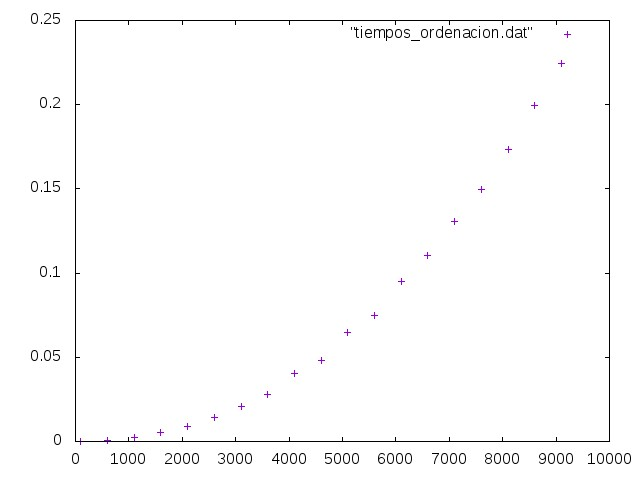
\includegraphics[width=0.8\textwidth]{grafica1_1.png}

\end{figure}


\subsection{Ejercicio 2: Ajuste en la ordenación de la burbuja}
Replique el experimento de ajuste por regresión a los resultados obtenidos en el ejercicio 1 que calculaba la eficiencia del algoritmo de ordenación de la burbuja. Para ello considere que f(x) es de la forma $a*x^2 + b*x + c$.

\subsection{Ejercicio 3: Problemas de precisión}
Junto con este guión se le ha suministrado un fichero ejercicio\_desc.cpp. En él se ha implementado un algoritmo. Se pide que:
\begin{itemize}
	\item Explique qué hace este algoritmo.
	\item Calcule su eficiencia teórica.
	\item Calcule su eficiencia empírica.
\end{itemize}
Si visualiza la eficiencia empírica debería notar algo anormal. Explíquelo y proponga una solución. Compruebe que su solución es correcta. Una vez resuelto el problema realice la regresión para ajustar la curva teórica a la empírica.

\subsection{Ejercicio 4: Mejor y peor caso}
Retome el ejercicio de ordenación mediante el algoritmo de la burbuja. Debe modificar el código que genera los datos de entrada para situarnos en dos escenarios diferentes:
\begin{itemize}
	\item El mejor caso posible. Para este algoritmo, si la entrada es un vector que ya está ordenado el tiempo de cómputo es menor ya que no tiene que intercambiar ningún elemento.
	\item El peor caso posible. Si la entrada es un vector ordenado en orden inverso estaremos en la peor situación posible ya que en cada iteración del bucle interno hay que hacer un intercambio.
\end{itemize}
Calcule la eficiencia empírica en ambos escenarios y compárela con el resultado del
ejercicio 1.

\subsection{Ejercicio 5: Dependencia de la implementación}
Considere esta otra implementación del algoritmo de la burbuja:
void ordenar(int *v, int n) {
bool cambio=true;
\begin{lstlisting}
void ordenar(int *v, int n) {
	for (int i=0; i<n-1 && cambio; i++) {
		cambio=false;
		for (int j=0; j<n-i-1; j++) {
			if (v[j]>v[j+1]) {
				cambio=true;
				int aux = v[j];
				v[j] = v[j+1];
				v[j+1] = aux;
			}
		}
	}
}
\end{lstlisting}
En ella se ha introducido una variable que permite saber si, en una de las iteraciones del
bucle externo no se ha modificado el vector. Si esto ocurre significa que ya está ordenado
y no hay que continuar.
Considere ahora la situación del mejor caso posible en la que el vector de entrada ya está
ordenado. ¿Cuál sería la eficiencia teórica en ese mejor caso? Muestre la gráfica con la
eficiencia empírica y compruebe si se ajusta a la previsión.

\subsection{Ejercicio 6: Influencia del proceso de compilación}
Retome el ejercicio de ordenación mediante el algoritmo de la burbuja. Ahora replique dicho ejercicio pero previamente deberá compilar el programa indicándole al compilador que optimice el código. Esto se consigue así:\\
\hspace*{2cm} \emph{g++ -O3 ordenacion.cpp -o ordenacion\_optimizado} \\
Compare las curvas de eficiencia empírica para ver cómo mejora esto la eficiencia del programa.

\subsection{Ejercicio 7: Multiplicación matricial}
Implemente un programa que realice la multiplicación de dos matrices bidimensionales. Realice un análisis completo de la eficiencia tal y como ha hecho en ejercicios anteriores de este guión.

\subsection{Ejercicio 8: Ordenación por Mezcla}
Estudie el código del algoritmo recursivo disponible en el fichero mergesort.cpp. En él, seintegran dos algoritmos de ordenación: inserción y mezcla (o mergesort). El parámetro UMBRAL\_MS condiciona el tamaño mínimo del vector para utilizar el algoritmo deinserción en vez de seguir aplicando de forma recursiva el mergesort. Como ya habráestudiado, la eficiencia teórica del mergesort es n log(n). Realice un análisis de la eficiencia empírica y haga el ajuste de ambas curvas. Incluya también, para este caso, un pequeño estudio de cómo afecta el parámetro UMBRAL\_MS a la eficiencia del algoritmo.Para ello, pruebe distintos valores del mismo y analice los resultados obtenidos.


\end{document}